\documentclass[11pt]{article}
\usepackage{natbib}
\usepackage{graphicx}
\usepackage{tikz}
\usetikzlibrary{shapes,arrows}
\usepackage{pdflscape}
\usepackage{hyperref}
\usepackage{multirow}
\usepackage{listings}
% Fonts for commands, etc.
\usepackage[scaled=0.92]{helvet}
\usepackage[scaled=0.92]{uarial}
 
% Default margins are too wide all the way around. I reset them here
\setlength{\topmargin}{-.5in}
\setlength{\textheight}{9in}
\setlength{\oddsidemargin}{.125in}
\setlength{\textwidth}{6.25in}
\setlength{\topmargin}{-.5in} 
\setlength{\textheight}{9in}
\setlength{\oddsidemargin}{.125in}
\setlength{\textwidth}{6.25in} 

% Define block styles for the flow diagrams used in the document
\tikzstyle{decision} = [diamond, draw, fill=blue!20, 
    text width=4.5em, text badly centered, node distance=3cm, inner sep=0pt]
\tikzstyle{block} = [rectangle, draw, fill=blue!20, 
    text width=5em, text centered, rounded corners, minimum height=4em]
\tikzstyle{line} = [draw, -latex']
\tikzstyle{cloud} = [draw, ellipse,fill=red!20, node distance=3cm,
    minimum height=2em]

% Super and Sub-script commands for text-mode
\newcommand{\superscript}[1]{\ensuremath{^{\textrm{#1}}}}
\newcommand{\subscript}[1]{\ensuremath{_{\textrm{#1}}}}
% Command to represent options for filterBam: "phv": helvetica, "pcr": courier ZapfChancery
\newcommand{\printOption}[1]{$\textrm{-\,-}${\fontfamily{phv}\selectfont#1}$\langle${\fontfamily{phv}\selectfont value}$\rangle$}
\newcommand{\setOption}[2]{{\fontfamily{phv}\selectfont#1}\ensuremath{=#2}} %{option}{value}
\newcommand{\option}[1]{{\fontfamily{phv}\selectfont#1}}
\newcommand{\bamApi}[1]{{\fontfamily{bch}\selectfont#1}}
\newcommand{\software}[1]{{\fontfamily{cmss}\selectfont#1}}
\newcommand{\unix}[1]{\texttt{#1}}
\newenvironment{cmdOutput}{\ttfamily}

% Setting up title, etc 
\title{Filtering read alignments in BAM format: user guide} 
\author{Tonatiuh Pe\~{n}a-Centeno \\
University of Greifswald}
\date{\today}

 
\begin{document}  
\maketitle
\abstract{This note documents "filterBAM", a program designed to clean alignments stored in BAM format. 
The filter is based on filterPSL, a perl script written by Prof. Mario Stanke as part of the AUGUSTUS 
software suite \citet{stanke08:augustus}. Both filterPSL and filterBam are designed for the cleaning of 
alignment data that will subsequently be applied to the gene prediction problem. The filter produces also 
output that might later be used for transcriptome quantification. The code should be modifiable rather 
easily, if it is to be applied to a different type of application. 
filterBam is written in C++ and makes use of the Bamtools API of \citet{barnett11:BamTools}. 

\section{Installation}

In this section we describe the system requirements for installing, compiling and running filterBam on a 
Linux terminal. 

\subsection{Requirements}
Table \ref{tab:software} and \ref{tab:libraries} below list the software packages and libraries required 
for compiling filterBam. As the filter works with sorted BAM files, it might be useful to have both 
\software{samtools} and \software{bamtools} utility kits installed, so both software packages have been 
included in the tables.

\begin{table}
  \begin{center}
    \begin{tabular}{|l|l|l|}
	\hline 
	\multicolumn{3}{|c|}{Software Dependencies} \\ \cline{1-3}
	\hline
      Name		& 	version	& Available at \\ \cline{1-3}
      Bamtools	&	2.1.0	& \url{https://github.com/pezmaster31/bamtools} \\ \cline{1-3}
      Samtools (optional)	& 	0.1.18	& \url{http://samtools.sourceforge.net/} \\ \cline{1-3}
    \end{tabular}
  \end{center}
  \caption{List of software required by filterBam}
  \label{tab:software}
\end{table}

\begin{table}
  \begin{center}
    \begin{tabular}{|l|l|l|l|}
	\hline
	\multicolumn{4}{|c|}{Library Dependencies} \\ \cline{1-4}
	\hline
	  Names		&  version  & Available at	&	Notes\\ \cline{1-4}
	  zlib		&  $>=$ 1.2.2.1 & \url{<http://www.zlib.net>} & For support of BGZF format\\ \cline{1-4}
    \end{tabular}
  \end{center}
  \caption{List of libraries required by filterBam}
  \label{tab:libraries}
\end{table}

Basic instructions on how to get and use the latest versions of \software{Samtools} and \software{Bamtools} 
are provided in Section \ref{sec:utilityKits}.

% Note that the flag \unix{-std=c++0x}  has been used given that some of the functionalities of the filter 
% require some of the newest features of GNU's g++ compiler. It seems that c++11 has bundled such 
% functionalities. 

\subsection{Compilation}

In this section we briefly describe the compilation process of \software{filterBam}. 

\begin{enumerate}
	\item
		Download or checkout the latest version of filterBam from \url{to-specify}. 
	\item
		Create and export an environment variable \unix{BAMTOOLS} that points to the folder where 
		\software{bamtools} has been installed. For example, if \software{bamtools} is under 
		\unix{/home/myAccount/}, then do the following: \unix{\$BAMTOOLS=/home/myAccount;} and then 
		\unix{\$export BAMTOOLS}. 		
	\item
		Move to the directory where filterBam has been installed and type \unix{make}. This should compile 
		the program filterBam.cc and the source of this document, filterBam.tex.
	\item
		The binary will be stored in \unix{filterBam/bin} and the documentation in \unix{filterBam/doc}. 
\end{enumerate}

\section{A couple of examples}
In this section we show how the filter works through the application of a couple of examples. The first 
example documents the operation of the filter for single alignments, while the second example describes 
the operation of the filter in paired-alignment mode. The filter accepts a \option{help} option to 
display its funcionalities.

\subsection{Dummy data}
We have generated two dummy data sets to show filterBam in operation. One file illustrates how the cleaning of
single alignments works, while the other file shows how paired alignments are processed. The file 
\unix{example\_single.bam} is a BAM file consists of a set of alignments that were specifically tailored to 
show the functionalities of the filter when treating inputs as single alignments. In a similar way, the file 
\unix{example\_paired.bam} was constructed with alignments that are product of paired-reads, so that the 
functionalities of the filter under this mode of operation are shown. Dummy data are stored under the folder 
\unix{filterBam/data}.

\subsection{Filtering of single alignments}
The filter allows screening out alignment under a set of different criteria: coverage level, percentage of 
identity and insert gaps, with default values specified in Table \ref{tab:featuresFilter}. Running the filter 
on \unix{example\_paired.bam} with default options, that is: 

\begin{flushleft}
  \begin{cmdOutput}
    > filterBam --in data/example\_1.bam --out data/example\_1.f.bam
  \end{cmdOutput}
\end{flushleft}

will lead to the following output: 

\begin{flushleft}
  \begin{cmdOutput}
    ------------------------------------- \\
    Summary of filtered alignments: \\
    ------------------------------------- \\ 
    unmapped        : 11 \\
    percent identity: 5 \\
    coverage        : 0 \\
    ------------------------------------- \\
    Cmd line: \\
    filterBam --in data/example\_1.bam --out data/example\_1.f.bam \\
    ------------------------------------- \\
    Elapsed time:   0 seconds. \\
  \end{cmdOutput}
\end{flushleft}

The source file, \unix{example\_1.bam} stores $35$ alignments, whereas the filtered output has $19$ alignments.
As the output shows, $16$ alignments were cleaned, $11$ because they were not mapped and $5$ because of the 
percent identity criteria. \\

Parameters of the filter might be modified. A run with \setOption{minCover}{70} will lead to a very different 
output. The options \option{best} and \option{uniq} are both mutually exclusive, because they make the filter 
let pass only alignments that have a minimum thresholding score.


\subsection{Filtering of paired alignments}
RNA-seq libraries might contain paired-reads, which provide additional information by means of the distance 
kept between the end of one read and the start of the other; something termed as the insert length. In fact,
aligners such as \software{Bowtie} and \software{GSNAP} allow the alignment of paired reads by simply 
using both sets of reads as inputs. Nevertheless, sets of single reads that have been aligned 
independently might also be used to extract pairedness information: simply look pairs of alignments that 
might be potential pair-mates. filterBam does precisely that, within a single BAM file; for further information
on how this is done see the Section \ref{sec:pairedAls}.

In order for the filter to work on the paired-alignment mode, the option \printOption{paired} must be set. The 
same set of options are available as with the single-alignment filter. However, there are subtle differences 
on the criteria \printOption{best} or \option{uniq}, which are explained in Section \ref{sec:pairedAls} of the 
reference manual.

\begin{flushleft}
  \begin{cmdOutput}
    ------------------------------------- \\ 
    Summary of filtered alignments:  \\
    -------------------------------------  \\
    unmapped        : 2 \\
    percent identity: 0 \\
    coverage        : 0 \\
    not paired      : 1 \\
    quantiles of unspliced insert lengths: [insertlen.size()=4]  \\
    q[10\%]=76,q[20\%]=76,q[30\%]=77,q[40\%]=77,q[50\%]=137,q[60\%]=137,q[70\%]=137,q[80\%]=138,q[90\%]=138, \\
    unique          : 2  \\
    -------------------------------------  \\
    Cmd line:  \\
    ./filterBam --in data/example\_paired.bam --out data/example\_paired.f.bam --paired --minId 70 --uniq --uniqThresh 0.99 --verbose  \\
    ----------------------------------------  \\
    Elapsed time:   0 seconds.  \\
  \end{cmdOutput}
\end{flushleft}

In this example, the file \unix{example\_paired.bam} originally with $7$ alignments is filtered under the 
paired alignment mode, and with the options \setOption{minId}{70} and \setOption{uniqThresh}{0.99}. Setting 
these parameters to such values will lead to the filter to discard $5$ alignments and to let pass only $2$.

\subsection{Common gene information}
When using paired alignments, an important source of information might be whether optimal alignments were 
aligned to a common target. The option \printOption{commonGeneFile} allows to store such type of information 
in a text file. 

\subsection{Pairdness coverage information}
For paired alignments, and in fact for paired reads, an important source of information is the distance kept 
between reads. When operating in paired-alignment mode, filterBam preserves the information of pairedness 
coverage between mate pairs. This feature is activated with the \printOption{pairBed}. 

\textbf{Warning}: At present time, the routine for collecting pairedness coverage information slows down quite 
a lot the execution time, so use it your own risk. Nevertheless, a faster version of this feature should be 
available relatively soon.

\subsection{Other}
This software has been tested on a a Dell (x86\_64) computer with Ubuntu 10.04 (lucid). Compilation of the 
code was done with GNU's C++ compiler, gcc version 4.4.3. 

\section{Technical specifications}

Other relevant issues that might be well documenting go here.

\subsection{Input data}
The filter should work fine for data coming from $454$ and Illumina technologies but not for colorspace data generated by SOLiD technology. 

\section{About Samtools and Bamtools} \label{sec:utilityKits}

We introduce some examples of how to use Samtools and Bamtools to make life easier when working with BAM files.
In particular we concentrate on the issue of sorting files by query name, as this is the requirement for 
filterBam. Attention should be paid to the fact that SAM and BAM files contain a header, so any sorting 
routine must consider the following: to momentarily put aside the header, do the sorting, and then insert the 
header at the top of the sorted file.
 
\subsection{Samtools}
\software{Samtools} is an API written in the \unix{C} language that includes a set of utilities for 
manipulating SAM/BAM files. The software is available via \software{subversion} on the web-page 
\url{http://samtools.sourceforge.net/}. Folow the installation instructions contained therein and a binary 
file \unix{samtools} will be produced. Some useful commands follow:

\begin{itemize}
	\item	Help
			\unix{samtools --help} 
	\item	Convert from SAM to BAM \\
			\unix{samtools view -bS input.sam -o output.bam} 
	\item	Convert from BAM to SAM \\
			\unix{samtools view -h input.bam > output.sam}
	\item	Sort BAM file \\
			\unix{samtools sort input.bam out}
\end{itemize}



\subsection{Bamtools}

In a similary way, \software{Bamtools} is an API, but now written in \unix{C++}, that also includes an 
utility-kit to manipulate BAM files. Get hold of the latest version of \software{Bamtools} by following 
the instructions contained in \url{https://github.com/pezmaster31/bamtools/wiki/Building-and-installing}; the 
software \software{git} will be required. After compilation, a binary \unix{bin/bamtools} will be created. 
Some of the commands useful commands are:

\begin{itemize} 
	\item	Help \\
			\unix{bamtools --help}			
	\item	Count number of alignments in a BAM file \\
			\unix{bamtools count -in input.bam}
	\item	Sorting files by query name [WARNING: it seems that this sorting does not behave well with 
			characters s.a. ":" ] \\
			\unix{bamtools sort -byname -in input.bam -out output.bam}
\end{itemize}


% We start a new section of the document, the "Reference Guide", so 
% it is worth changing the name of the document and make a new title, 
% in a new page
\newpage
\begin{center}
{\LARGE Filtering read alignments in BAM format: reference manual}
\end{center}

\begin{center}
{\large
Tonatiuh Pe\~{n}a-Centeno \\ 
\date{\today}
}
\end{center}

\abstract{This note describes the detailed operation of the filter and lists the main classes that were used to 
implement it. In this way, people in the future might improve or reuse the filterBam code for other 
type of applications}. 

\section{Introduction}
RNA-seq data has become an important source of information for tasks such as differential 
expression analysis, transcript quantification and gene prediction. Given that this new technology 
produces millions of such short-reads ($\sim30bp$), bespoke methods and tools are required to process such big 
amounts of information. For example, a single run of an RNAseq experiment will produce millions, if not, 
hundreds of millions of short reads [Ref: Wiki].

After sequencing and generation of an RNAseq dataset, a later step consists of utilising the short 
reads to obtain an approximate 
version of the transcriptome, typically via the alignment of the reads to a reference genome. 
Such alignments can be carried out with tools such as BLAT, Bowtie, GSNAP, among others. In particular, 
Bowtie and GSNAP are specifically designed to align reads as short as $50$ and $14$ bp, respectively. 
Very recently, the introduction of the Sequence AlignMent Format, or SAM, by \citet{heng09:SAM}, has meant 
that many of the aforementioned alignment tools now produce outputs in SAM format. 

filterBam is a C++ code that cleans alignment files stored in BAM format, which is the binary version of 
SAM. The software package is based on filterPSL, a Perl routine written by Prof. Dr. Mario Stanke for the processing of 
alignment records stored in PSL format. filterPSL is part of a set of Perl scripts that accompany the 
distribution of the annotation software, AUGUSTUS [Ref]. filterPSL is mainly used as a preprocessing step 
for cleaning alignments obtained with softwares such as BLAT, and filterBam is supposed to supersede 
it by doing the same task but on RNAseq alignment data stored in a BAM file. 

\section{Main features}

In a nutshell, assuming a BAM file given as input, filterBam by default cleans all those alignments that are either unmapped or do not satisfy any of the following conditions:  
\begin{enumerate}
	\item	do not comply with a minimum coverage;
	\item	do not have a minimum value of percentage identitiy, or 
	\item	(optionally), do not satisfy a minimum value of base inserts. 
\end{enumerate} 
Table \ref{tab:featuresFilter} above summarises the main features of the filter. 

\begin{table}
  \begin{center}
    \begin{tabular} {|c|c|c|c|} \hline
	 \multicolumn{4}{|c|}{\textbf{filterBam}} \\ \hline
      Action & Feature & Option & Default value \\ \hline 
      \multicolumn{4}{|c|}{Every alignment} \\ \hline
      \multirow{4}{*}{Screens out} & unmapped & -- &  -- \\ \cline{2-4}
      & coverage level & minCover & 80\% \\  \cline{2-4}
      & pctge identity & minId & 92\%\\  \cline{2-4}
      & insert gaps & insertLimit & 10bp\\ \hline
      \multicolumn{4}{|c|}{Single alingments} \\ \hline
      \multirow{2}{*}{Screens out} & best & -- & nore \\ \cline{2-4}
      & unique & uniqThresh & 0.96 \\ \hline
      \multicolumn{4}{|c|}{Paired alignments} \\ \hline
      \multirow{2}{*}{Screens out} & best & & \\  \cline{2-4}
      & uniq & uniqThresh & 0.96 \\ \hline
      \multirow{2}{*}{Writes to file} & common target genes & commonGeneFile & false \\  \cline{2-4} 
      & pairedness coverage info & pairBedFile & false \\ \hline
    \end{tabular}
    \caption{Main features of filterBam.}
    \label{tab:featuresFilter}
  \end{center}
\end{table}

After this basic set of filters has been applied, the alignments are processed according to whether they 
originated from single- or paired- RNAseq reads. Single alignments are cleaned by droppping out all those 
that do not satisfy a score value that depends on the coverage and the percentage identity of the aligned read,
i.e. $score(coverage, percId)$. Paired alignments are mated to other alignments according to the distance and 
insert length from their associated reads; the filter then drops out all those pairs of alignments that do 
not satisfy a score value that, once again, depends on coverage and percentage identity, ($score(coverage, percId)$).
 
The subsequent sections of this document describe in a step-wise manner how the filtering of single- and 
paired-alignments is done. The basic set of filters is described in Section \ref{sec:basicFilters}. 
Then the filtering of single alignments is explained in Section \ref{sec:singleAls}, and finally the filtering 
of paired alignments is explained in Section \ref{sec:pairedAls}.
 
 
\section{Basic filters} \label{sec:basicFilters}
Figure \ref{tik:singleFilter} below shows the schematics of the operation of the filter for single 
alignments. In the subsequent, we will assume an input BAM file is constituted by a series of records 
$i=\{1,\dots,N\}$, each containing the information of an alignment. See \citep{heng09:SAM} for further 
reference. The filter first checks whether 
alignment $i$ is mapped or not, and this is easily done by means of verifying the bit $0\times4$ of the 
alignment FLAG (SAM field number 2). As the specification suggests, this bit is the only source 
of reliable information to determine whether a read is mapped or not \citet{heng09:SAM}. This verification 
is achieved by using the \bamApi{isMapped} method of BamTools. Unmapped reads are dropped, while mapped 
reads continue further processing. A counter keeps track of the number of unmapped reads that were dropped. 

As a second step, alignments that passed the mapping test are appended with two additional but temporary 
string-tags. Tag `co' and tag `pi' are added to the binary alignment by the \bamApi{addTag} method of BamTools. 
`co' stands for \emph{coverage} and is a measure of the amount of reads located at a given genomic position. 
`pi' stands for \emph{percentage identity} and is a measure of the number of basis that correctly identify 
a genomic position. Estimation of the coverage is done according to Equation \ref{eq:coverage}, whilst 
estimation of the percentage identity is done following Equation \ref{eq:percId}, both in the Appendix. 

If the estimated coverage value for the read in alignment $i$ is less than that of the specified 
\option{minCover}, the alignment will be dropped and a counter keeping track of such types of events will 
be updated. In a similar way, if the value of \option{percId} for the read of alignment $i$, is less than that 
specified by \option{minId}, the alignment will be dropped and the corresponding counter will be updated. 
Default values for \option{minCover} and \option{percId} are shown in Table \ref{tab:featuresFilter} 
respectively, but might be modified by using the options \printOption{minCover} and \printOption{minId}.


\section{Single alignments} \label{sec:singleAls}
Continuing with Figure \ref{tik:singleReadFilter}, we assume either options \option{best} or \option{uniq}  
are selected, but not option \option{paired}. The core issue to understand in the operation of the single-
alignment mode filter, is that batches of alignments belonging to a common query QNAME\subscript{1} will 
be processed independently from alignments belonging to a different query name QNAME\subscript{2}. 

Alignments that passed the mapping test are appended with two additional but temporary 
string-tags. Tag $co$ and tag $pi$ are added to the binary alignment by means of the \bamApi{addTag} method of 
BamTools. Tag $co$ stands for \emph{coverage} and is a measure of the amount of reads located at a given 
genomic position. Meanwhile $pi$ stands for \emph{percentage identity} and is a measure of the number of 
basis that correctly identify a genomic position. Whereas estimation of the coverage is done according to 
Equation \ref{eq:coverage}, estimation of the percentage identity is done according to Equation \ref{eq:percId}, both in the Appendix. Table \ref{tab:singleReads} below shows a series of alignments with the $co$ and 
$pi$ tags added.

 
If the estimated coverage value of alignment $i$ is less than that of \option{minCover}, the alignment 
will be dropped and a counter keeping track of such types of drops will be updated. In a similar way, if 
the value of \option{percId} for alignment $i$, is less than that specified by \option{minId}, the read 
will be dropped and the corresponding counter will be updated. Default values for \setOption{minCover}{80} 
and \setOption{percId}{92} might be modified by using the options \printOption{minCover} and 
\printOption{minId}, respectively.

An optional value, the number of inserts to the base reference (baseInsert), is computed optionally if 
the '--noIntrons' option is used. The number of insertions to the reference is computed through the 
application of Equation \ref{eq:baseInsert}. This filter depends on the insertLimit value that has been 
specified, and which by default has a value of $10$. The insertLimit parameter might be modifed by 
applying the \printOption{insertLimit} option.

\begin{figure}
\begin{center}
  \begin{tikzpicture}[node distance=1mm, auto,
    decision/.style={diamond, draw=black, thick, fill=white,
    text width=4em, text badly centered,
    inner sep=1pt, font=\sffamily\small},
    block_center/.style ={rectangle, draw=black, thick, %fill=white,
      text width=8em, text centered, minimum height=3em},
    block_left/.style ={rectangle, draw=black, thick, fill=white,
      text width=16em, text ragged, minimum height=3em, inner sep=6pt},
    block_noborder/.style ={rectangle, draw=none, thick, fill=none,
      text width=18em, text centered, minimum height=1em},
    block_assign/.style ={rectangle, draw=black, thick, fill=white,
      text width=18em, text ragged, minimum height=3em, inner sep=6pt},
    block_lost/.style ={rectangle, draw=black, thick, fill=white,
      text width=16em, text ragged, minimum height=3em, inner sep=6pt},
      line/.style ={draw, thick, -latex', shorten >=0pt}]

    % outlining the flowchart using the PGF/TikZ matrix funtion
    \matrix [column sep=12mm,row sep=3mm] {

    % Place nodes
    \node [cloud] (Start) {Start}; & & \node [cloud] (alpha2) {$\alpha$}; \\ 
	\node [decision] (unmapped) {Unmapped?}; & & \node [block_center] (scoreAli) {Score alignments}; \\
    \node [block_center] (percId) {Percentage identity (percId)}; & & \node [decision] (unique) {Unique?}; \\
	\node [decision] (ifPercId) {percId$\ge$minId?}; & & \node [block_center] (similar) {Similarity}; \\
    \node [block_center] (coverage) {Coverage (coverage)}; & & \node [decision] (ratio) {ratio\\(top,second)}; \\
	\node [decision] (ifCoverage) {coverage\\$\ge$\\minCover?}; & & \node [block_center] (top){Select top alignment}; & \node [block_center] (best) {Select align's sharing top score}; \\

    \node [decision] (noIntrons) {noIntrons?}; & \node [decision] (insertLimit) {baseInsert $<$ insertLimit?}; & \node [block_center] (save) {Save alignments};  \\
     \node [decision] (addOptions) {Unique\\$~\mathbf{|}~$\\Best?}; &  \node [block_center] (baseInsert) {Base inserts}; & \node [cloud] (end) {End}; & \\
    \node [cloud] (alpha) {$\alpha$}; & & \\
};% end matrix

    \begin{scope}[every path/.style=line]
	% Drawing paths, starting from left-most column

    % paths from the first column
    \path [line] (Start) -- (unmapped);
    \path  (unmapped) -- node {no} (percId);
	\path  (percId) -- (ifPercId);
    \path  (ifPercId) -- node {yes} (coverage);
	\path  (coverage) -- (ifCoverage);
    \path  (ifCoverage) -- node {yes} (noIntrons);
    \path  (noIntrons) -- node {no} (addOptions);
    \path  (insertLimit) -- (baseInsert);
    \path  (baseInsert) -- (addOptions);
    \path [line,dashed] (addOptions) -- node {yes} (alpha);  
	
	% paths from the second column
	\path (noIntrons) -- (insertLimit);
	%% \path (insertLimit) -| (addOptions);

	% paths from the third column
	\path (alpha2) -- (scoreAli);
	\path (scoreAli) -- (unique);
	\path (unique) -- (similar);
	\path (similar) -- (ratio);
	\path (ratio) -- (top);
	\path (top) -- (save);
	\path (save) -- (end);

	% paths from the fourth column
	\path (unique) -| (best);
	\path (best) |- (save);

   \end{scope}

  \end{tikzpicture}
  % Caption and label
  \caption{Flow diagram of the operation of the single-read filter}
  \label{tik:singleFilter}
\end{center}
\end{figure}

\subsection{Uniq and Best criteria}
Further cleaning can be achieved by means of selecting the mutually exclusive \option{unique} or 
\option{best} options. If such is the case, Figure \ref{tik:singleFilter} shows how an alignment record 
continues throughout the process path. Options \option{best} and \option{unique} stand for the filter 
selecting the \emph{best} group of alignments, or the single-top alignment (i.e. \option{unique}), in terms 
of a cost function, which in this case is given defining the expression 

\begin{equation}
	\mathrm{score} = \mathrm{percId} + \mathrm{coverage}.
\label{eq:score}
\end{equation}

Thus, after an alignment has passed through the mapping, coverage, percentage identity and intron-gap 
filters, the information from coverage and percentage identity is be combined into the figure \option{score}.
Such value is added to the alignment as the tag $sc$. 

After a group of alingments belonging to the same query has been scored, the group is sorted by such score 
value; as illustrated in Tables \ref{tab:singleReads} and \ref{tab:sortedReads} below.

\begin{landscape}
  \begin{table}\footnotesize
\begin{center}
    \begin{tabular*}{0.75\textwidth}{|l|l|l|l|l|l|l|}
	\cline{1-7}
	  QNAME & RNAME & startPOS & endPOS & pi & co & sc \\ \cline{1-7}
      r2/1 & chr17 & 27698729 & 27698778 & 98 & 100 & 198 \\ \cline{1-7}
      r2/1 & chr17 & 20320140 & 20320189 & 94 & 100 & 194 \\ \cline{1-7}
      r2/1 & chr19 & 1364 & 1413 & 98 & 100 & 198 \\ \cline{1-7}
      r2/1 & chr17 & 8038458 & 8038507 & 96 & 100 & 196 \\ \cline{1-7}
      r2/1 & chr17 & 24524223 & 24524271 & 94 & 100 & 194 \\ \cline{1-7}
      r2/1 & chr17 & 30676704 & 30676750 & 96 & 96 & 192 \\ \cline{1-7}
      r2/1 & chr17 & 16894327 & 16894376 & 94 & 100 & 194 \\ \cline{1-7}
      r2/1 & chr17 & 5031882 & 5031931 & 96 & 100 & 196 \\ \cline{1-7}
      r2/1 & chr18 & 0 & 49 & 98 & 100 & 198 \\ \cline{1-7}
    \end{tabular*}
    \caption{SAM alignments with added tags: percId, coverage and score}
    \label{tab:singleReads}
\end{center}
  \end{table}

  %%%%%%%%%%%%%%%%%%%%%%%%%%%%%%%%%%%%%%%%%%%%%%%

  \begin{table}\footnotesize
\begin{center}
    \begin{tabular*}{0.75\textwidth}{|l|l|l|l|l|l|l|}
	\cline{1-7}
	  QNAME & RNAME & startPOS & endPOS & pi & co & sc \\ \cline{1-7}
      r2/1 & chr17 & 27698729 & 27698778 & 98 & 100 & 198 \\ \cline{1-7}
      r2/1 & chr19 & 1364 & 1413 & 98 & 100 & 198 \\ \cline{1-7}
      r2/1 & chr18 & 0 & 49 & 98 & 100 & 198 \\ \cline{1-7}
      r2/1 & chr17 & 8038458 & 8038507 & 96 & 100 & 196 \\ \cline{1-7}
      r2/1 & chr17 & 5031882 & 5031931 & 96 & 100 & 196 \\ \cline{1-7}
      r2/1 & chr17 & 20320140 & 20320189 & 94 & 100 & 194 \\ \cline{1-7}
      r2/1 & chr17 & 24524223 & 24524271 & 94 & 100 & 194 \\ \cline{1-7}
      r2/1 & chr17 & 16894327 & 16894376 & 94 & 100 & 194 \\ \cline{1-7}
      r2/1 & chr17 & 30676704 & 30676750 & 96 & 96 & 192 \\ \cline{1-7}
    \end{tabular*}
    \caption{SAM alignments after sorting by score}
    \label{tab:sortedReads}
\end{center}
  \end{table}

\end{landscape}

The difference between the \option{uniq} and \option{best} criteria is that the former will select only 
the top-scored alignment and will write it into file. Table \ref{tab:sortedReads} shows the same set of 
alignments as in Table \ref{tab:singleReads}, but after ranking by score. According to the \option{best} 
criterion, only the alignmnents sharing the optimal score will be preserved, while the rest of suboptimal 
alignments will be dropped. In the example of Table \ref{tab:sortedReads}, the alignments sharing the 
score=$198$ will be preserved while the rest will be discarded. 

The option \option{uniq} is based also on the sorting of alignments by its score. The main difference however 
is that only one alignment is preserved, provided that it is one of those sharing the top score, but also 
provided that it is  is elligible to be preserved. However, in case a group of alignments happen to share 
the same score, filterBam checks whether such alignments are similar; whereby similarity refers to two 
reads to have been aligned on overlapping positions. 

\subsection{Similarity function}
A function that tests whether alignments (or two alignment pairs) are similar has been included within 
filterBam. Testing for similarity is required given that by handling separately spliced and unspliced 
alignments, there is the possibility that very similar alignments are reported, \emph{an unspliced read going approximately up to an intron and a spliced read with a few base pairs on one exon.} Such type of cases 
should not be considerd ambiguous when \option{uniq} is specified. 
  
Figure \ref{fig:similarityFunction} below shows two scenarios. In scenario one, a pair of reads were aligned 
to overlapping ranges of the reference genome; both reads are deemed similar. In scenario two, the reads 
are aligned to non-contiguous ranges of the reference genome, thus are considered not-similar.

\begin{figure}
  \begin{center}
    \includegraphics[width=7cm]{figures/similarityFunction.eps}
  \end{center}
\caption{The similarity function checks whether mate paired reads are overlapping or not.}
\label{fig:similarityFunction}
\end{figure}
 
Thus to finalise, a top-scored alignment will be let pass by the filter, if and only if, the second ranked 
alignment is not all too-similar to the top alignment.

\section{Paired alignments} \label{sec:pairedAls}

This section describes the filtering of paired alignments. This feature is enabled by selecting the option  
\option{paired}. By doing so, filterBam will compare a set of alignments belonging to a common query and 
determine which alignments are paired with which others. Such matching is done by examining the distance and 
insert length between candidate pairs. A more thorough explanation follows, nevertheless it is worth 
pointing out that before alignments are processed as paired alignments, they are subjected to the basic 
filters described in Section \ref{sec:basicFilters}. A flow chart of the operation of filterBam for paired 
alignments is shown in Figure \ref{tik:matePairFilter} below.


\begin{figure}
\begin{center}
  \begin{tikzpicture}[node distance=1mm, auto,
    decision/.style={diamond, draw=black, thick, fill=white,
    text width=4em, text badly centered,
    inner sep=1pt, font=\sffamily\small},
    block_center/.style ={rectangle, draw=black, thick, %fill=white,
      text width=8em, text centered, minimum height=3em},
    block_left/.style ={rectangle, draw=black, thick, fill=white,
      text width=16em, text ragged, minimum height=3em, inner sep=6pt},
    block_noborder/.style ={rectangle, draw=none, thick, fill=none,
      text width=18em, text centered, minimum height=1em},
    block_assign/.style ={rectangle, draw=black, thick, fill=white,
      text width=18em, text ragged, minimum height=3em, inner sep=6pt},
    block_lost/.style ={rectangle, draw=black, thick, fill=white,
      text width=16em, text ragged, minimum height=3em, inner sep=6pt},
      line/.style ={draw, thick, -latex', shorten >=0pt}]

    % outlining the flowchart using the PGF/TikZ matrix funtion
    \matrix [column sep=12mm,row sep=3mm] {

    % Place nodes
    \node [cloud] (Start) {Start}; & & \node [cloud] (alpha2) {$\alpha$}; & \\ 
	\node [decision] (unmapped) {Unmapped?}; & & \node [block_center] (scoreAli) {Score alignments}; & \\
	& & \node [block_center] (matePairs) {Compute mate pairs}; & \\
    \node [block_center] (percId) {Percentage identity (percId)}; & & \node [decision] (unique) {Unique?}; & \\
	\node [decision] (ifPercId) {percId$\ge$minId?}; & & \node [block_center] (similar) {Similarity btwn pairs}; & \\
    \node [block_center] (coverage) {Coverage (coverage)}; & & \node [decision] (ratio) {ratio\\(top,second)}; & \\
	\node [decision] (ifCoverage) {coverage\\$\ge$\\minCover?}; & & \node [block_center] (top){Select top mate-pair}; & \node [block_center] (best) {Select mate-pairs sharing top score}; \\

    \node [decision] (noIntrons) {noIntrons?}; & \node [decision] (insertLimit) {baseInsert $<$ insertLimit?}; & \node [block_center] (save) {Save alignments belonging to selected mate-pairs}; & \\
     \node [decision] (addOptions) {Unique\\$~\mathbf{|}~$\\Best?}; &  \node [block_center] (baseInsert) {Base inserts}; & \node [cloud] (end) {End}; & \\
    \node [cloud] (alpha) {$\alpha$}; & & & \\
};% end matrix

    \begin{scope}[every path/.style=line]
	% Drawing paths, starting from left-most column

    % paths from the first column
    \path [line] (Start) -- (unmapped);
    \path  (unmapped) -- node {no} (percId);
	\path  (percId) -- (ifPercId);
    \path  (ifPercId) -- node {yes} (coverage);
	\path  (coverage) -- (ifCoverage);
    \path  (ifCoverage) -- node {yes} (noIntrons);
    \path  (noIntrons) -- node {no} (addOptions);
    \path  (insertLimit) -- (baseInsert);
    \path  (baseInsert) -- (addOptions);
    \path [line,dashed] (addOptions) -- node {yes} (alpha);  
	
	% paths from the second column
	\path (noIntrons) -- (insertLimit);

	% paths from the third column
	\path (alpha2) -- (scoreAli);
	\path (scoreAli) -- (matePairs);
	\path (matePairs) -- (unique);
	\path (unique) -- (similar);
	\path (similar) -- (ratio);
	\path (ratio) -- (top);
	\path (top) -- (save);
	\path (save) -- (end);

	% paths from the fourth column
	\path (unique) -| (best);
	\path (best) |- (save);

   \end{scope}

  \end{tikzpicture}
  % Caption and label
  \caption{Flow diagram of the operation of the single-read filter}
  \label{tik:matePairFilter}
\end{center}
\end{figure}

 
\subsection{Mate pairs}

Figure \ref{fig:pairedReads} shows a diagram in which four reads have been aligned: rs.1 (71), rs.2 (72), 
rs.2 (139) and rs.1 (202); with starting positions between parentheses. Bare in mind that query names have 
been made to coincide, in order to facilitate the understanding of the matching process. We recall that 
filterBam accepts inputs with '/1', '/2' suffix when the option \option{paired} has been selected.

\begin{figure}
  \begin{center}
    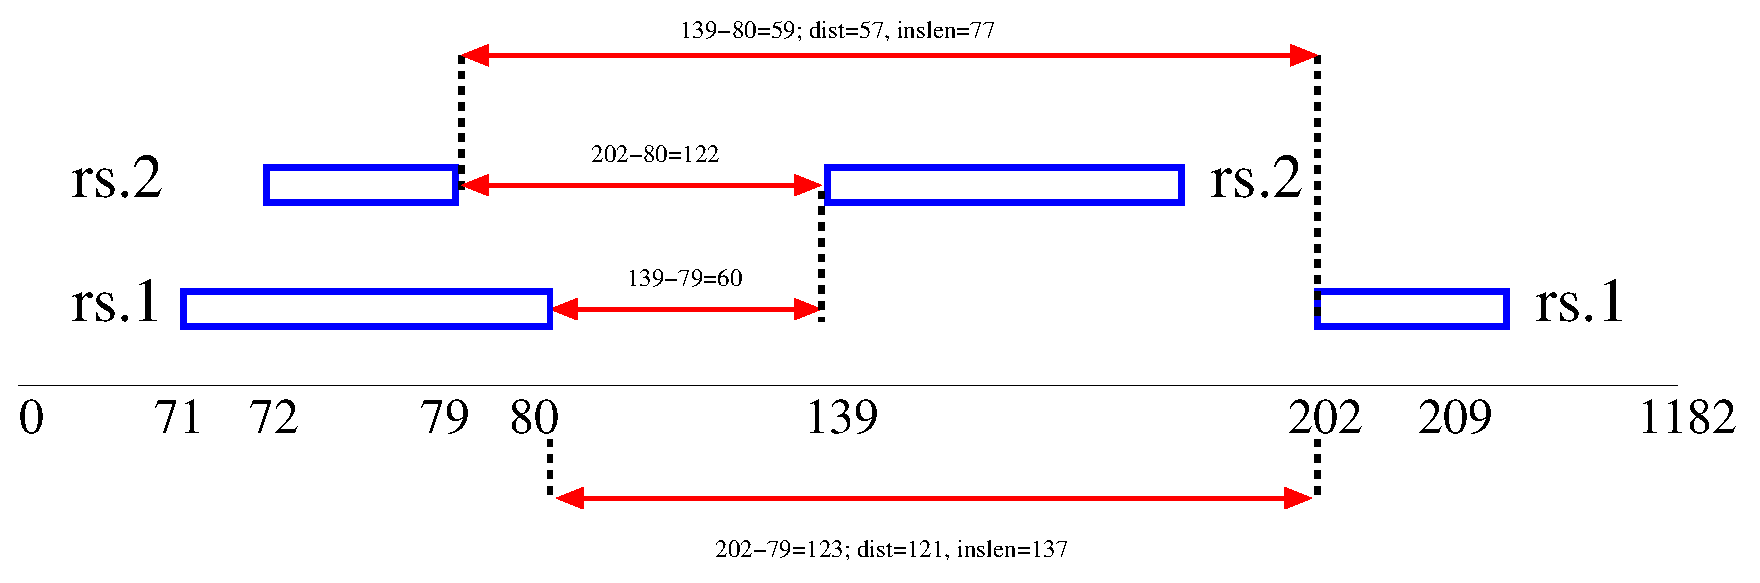
\includegraphics[scale=0.50]{figures/pairedReads.eps}
  \end{center}
\caption{Paired reads}
\label{fig:pairedReads}
\end{figure}

Within a group of alignments, presented in the example as queries $rs$, filterBam defines a list of candidate 
mate pairs, as shown in Table X below. If one pair of alignments belongs to different mates {1,2} and come 
from different strands {+,-}, then their distance and insert-length is computed. If a pair of alignments 
has $dist\ge 0 $ and $insLen\le maxInsertLimit$, the alignments are considered a valid mate-pair.

\begin{table}
\begin{center}
\begin{tabular}{|c|c|c|c|c|c|c|}\hline
	Mate 1 & Mate 2 & Strand 1 & Strand 2 & dist & insLen & score \\ \cline{1-7}
	rs1/1 (70) & rs1/1 (71) & false & false & -- & -- & -- \\ \cline{1-7}
	rs1/1 (70) & rs1/2 (138) & false & true & 57 & 77 & 3.8 \\ \cline{1-7}
	rs1/1 (70) & rs1/2 (201) & false & true & 120 & 138 & 3.875 \\ \cline{1-7}
	rs1/1 (70) & rs1/2 (499) & false & false & -- & -- & -- \\ \cline{1-7}
	rs1/1 (71) & rs1/2 (138) & false & true & 58 & 76 & 3.55 \\ \cline{1-7}
	rs1/1 (71) & rs1/2 (201) & false & true & 121 & 137 & 3.625 \\ \cline{1-7}
	rs1/1 (71) & rs1/2 (499) & false & false & -- & -- & -- \\ \cline{1-7}
	rs1/2 (138) & rs1/2 (201) & true & true & -- & -- & -- \\ \cline{1-7}
	rs1/2 (138) & rs1/2 (499) & true & false & -- & -- & -- \\ \cline{1-7}
	rs1/2 (201) & rs1/2 (499) & true & false & -- & -- & -- \\ \cline{1-7}
\end{tabular}
\label{tab:}
\caption{Candidate mate pairs in the example presented in Section \ref{sec:pairedAls}}
\end{center}
\end{table}    

\subsection{Uniq and Best criteria}

Figure \ref{tik:matePairFilter} shows the flow chart of operation of filterBam for paired alignments. 
As it can be seen, the filter operates under very similar tenets to those of the filter for single 
alignments, the main difference being that under the \option{paired} option, alignments are processed in 
pairs. Thus after scoring of the alignments of forming of the mate-pairs, the \option{uniq} selects the 
top-ranked pair of mates; where the rank is given by a function that makes use of the $coverage$ and 
$percId$ in very similar terms to those of Equation \ref{eq:score}. Analogously as well, the option 
\option{best}, lets pass the set of mate-pairs that share the maximum score. It is important to remark 
that alignments that were not paired are dropped. 


\section{Coverage, percent of identity and insert length}
The coverage is computed as the sum of the alignment matches (sequence matches or mismatches) and 
the insertions to the reference. Both figures, alignment matches and insertions to the reference, correspond 
to CIGAR string operations $M$ and $I$, respectively. Thus the following is done 

\begin{equation}
	\mathrm{coverage} = \frac{\sum\mathrm{CIGAR}\left(M,I\right)}{qLength}
	\label{eq:coverage}
\end{equation}

An approximation to the percentage of identity is given by computing the query length and subtracting the 
so-called edit distance to the reference (tag ``NM'' in SAM jargon), i.e.

\begin{equation}
	\mathrm{percId} = \frac{qLength - \mathrm{Tag}(NM)}{qLength}
	\label{eq:percId}
\end{equation}

The length of inserts is estimated by summing CIGAR operations ``M'' and ``I'', which correspond to alingment 
matches and deletions from the reference. In other words, we do the following

\begin{equation}
	\mathrm{InsertSize} = \frac{\sum\mathrm{CIGAR}\left(D,I\right)}{qLength}
	\label{eq:baseInsert}
\end{equation}


\begin{thebibliography}{1}
\providecommand{\natexlab}[1]{#1}
\providecommand{\url}[1]{\texttt{#1}}
\expandafter\ifx\csname urlstyle\endcsname\relax
  \providecommand{\doi}[1]{doi: #1}\else
  \providecommand{\doi}{doi: \begingroup \urlstyle{rm}\Url}\fi
 
\bibitem[Li et~al.(2009)Li, Handsaker, Wysoker, Fennell, Ruan, Homer, Math,
  Abecasis, Durbin, and Subgroup]{heng09:SAM}
H.~Li, B.~Handsaker, A.~Wysoker, T.~Fennell, J.~Ruan, N.~Homer, G.~Math,
  G.~Abecasis, R.~Durbin, and .~G. P. D.~P. Subgroup.
\newblock The sequence alignment/map format and samtools.
\newblock \emph{Bioinformatics Applications Note}, 25\penalty0 (16):\penalty0
  2078--2079, 2009.

\bibitem[Barnett et~al.(2011)Barnett, Garrison, Quinlan, Strömberg and Marth]{barnett11:BamTools}
D.~Barnett, E.~Garrison, A.~Quinlan, M.~Strömberg, G.~Marth.
\newblock BamTools: a C++ API and toolkit for analyzing and managing BAM files.
\newblock \emph{Bioinformatics}, 27\penalty0 (12):\penalty0
  1691-1692, 2011.

\bibitem[Stanke et~al.(2008)Stanke, Diekhans, Baertsch and Haussler]{stanke08:augustus}
M.~Stanke, M.~Diekhans, R.~Baertsch, D.~Haussler.
\newblock Using native and syntenically mapped cDNA alignments to improve de novo gene finding.
\newblock doi: 10.1093/bioinformatics/btn013

\end{thebibliography}

%\bibliographystyle{abbrvnat}

\end{document}
